\documentclass[11pt]{article}

\usepackage[a4paper,margin=0.88in]{geometry}
\usepackage[T1]{fontenc}
\usepackage[utf8]{inputenc}
\usepackage{lmodern}
\usepackage{microtype}
\usepackage{amsmath,amssymb,mathtools}
\usepackage{booktabs,array}
\usepackage{graphicx}
\usepackage{enumitem}
\usepackage{xcolor}
\usepackage[hidelinks]{hyperref}

\emergencystretch=2em
\graphicspath{{../figures/}}
% Auto-generated by scripts/420_generate_pandrosion_420_paper_assets.py
\newcommand{\RowsCount}{20}
\newcommand{\BenchDevice}{mps}
\newcommand{\BenchTorch}{2.12.0}
\newcommand{\BenchNumpy}{2.4.4}
\newcommand{\QBestSpeedup}{70.66}
\newcommand{\QBestN}{4096}
\newcommand{\QBestDim}{25}
\newcommand{\PtwoBestSpeedup}{31.37}
\newcommand{\PtwoBestN}{4096}
\newcommand{\PtwoBestDim}{50}
\newcommand{\PthreeBestSpeedup}{15.26}
\newcommand{\PthreeBestN}{4096}
\newcommand{\PthreeBestDim}{100}
\newcommand{\MaxRelError}{4.34\times 10^{-15}}
\newcommand{\PtwoMaxRelError}{4.34\times 10^{-15}}
\newcommand{\PthreeMaxRelError}{2.26\times 10^{-15}}

\newcommand{\CascadeTableRows}{%
q active & 512 & 19/63 & 19 & 0.039 & 0.204 & 5.22 & 0.178 & 4.55 & 7.82e-16 \\
q active & 1024 & 21/88 & 21 & 0.054 & 0.341 & 6.36 & 0.227 & 4.24 & 1.26e-15 \\
q active & 2048 & 23/125 & 23 & 0.088 & 1.582 & 17.91 & 0.399 & 4.52 & 1.90e-15 \\
q active & 4096 & 25/176 & 25 & 0.159 & 11.248 & 70.66 & 1.130 & 7.10 & 2.58e-15 \\
partial stage 2 & 512 & 19/63 & 38 & 0.067 & 0.204 & 3.06 & 0.178 & 2.67 & 8.66e-16 \\
partial stage 2 & 1024 & 21/88 & 42 & 0.103 & 0.341 & 3.31 & 0.227 & 2.20 & 9.58e-16 \\
partial stage 2 & 2048 & 23/125 & 46 & 0.244 & 1.582 & 7.24 & 0.399 & 1.83 & 3.35e-15 \\
partial stage 2 & 4096 & 25/176 & 50 & 0.361 & 11.248 & 31.37 & 1.130 & 3.15 & 4.34e-15 \\
partial stage 3 & 512 & 19/63 & 63 & 0.106 & 0.204 & 1.93 & 0.178 & 1.69 & 5.78e-16 \\
partial stage 3 & 1024 & 21/88 & 84 & 0.161 & 0.341 & 2.12 & 0.227 & 1.41 & 1.33e-15 \\
partial stage 3 & 2048 & 23/125 & 92 & 0.428 & 1.582 & 4.32 & 0.399 & 1.09 & 1.45e-15 \\
partial stage 3 & 4096 & 25/176 & 100 & 0.737 & 11.248 & 15.26 & 1.130 & 1.53 & 2.26e-15 \\
random full n & 512 & 19/63 & 512 & 0.266 & 0.204 & 0.77 & 0.178 & 0.67 & 0.00e+00 \\
random full n & 1024 & 21/88 & 1024 & 1.427 & 0.341 & 0.24 & 0.227 & 0.16 & 0.00e+00 \\
random full n & 2048 & 23/125 & 2048 & 5.695 & 1.582 & 0.28 & 0.399 & 0.07 & 0.00e+00 \\
random full n & 4096 & 25/176 & 4096 & 20.664 & 11.248 & 0.54 & 1.130 & 0.05 & 0.00e+00 \\
}

\newcommand{\MiddleCascadeRows}{%
partial stage 2 & 128 & 15/32 & 30 & 30 & 0.047 & 5.22 & 3.05 & 4.82e-16 \\
partial stage 2 & 512 & 19/63 & 38 & 38 & 0.067 & 3.06 & 2.67 & 8.66e-16 \\
partial stage 2 & 1024 & 21/88 & 42 & 42 & 0.103 & 3.31 & 2.20 & 9.58e-16 \\
partial stage 2 & 2048 & 23/125 & 46 & 46 & 0.244 & 7.24 & 1.83 & 3.35e-15 \\
partial stage 2 & 4096 & 25/176 & 50 & 50 & 0.361 & 31.37 & 3.15 & 4.34e-15 \\
partial stage 3 & 128 & 15/32 & 32 & 32 & 0.089 & 3.21 & 1.88 & 5.11e-16 \\
partial stage 3 & 512 & 19/63 & 63 & 63 & 0.106 & 1.93 & 1.69 & 5.78e-16 \\
partial stage 3 & 1024 & 21/88 & 84 & 84 & 0.161 & 2.12 & 1.41 & 1.33e-15 \\
partial stage 3 & 2048 & 23/125 & 92 & 92 & 0.428 & 4.32 & 1.09 & 1.45e-15 \\
partial stage 3 & 4096 & 25/176 & 100 & 100 & 0.737 & 15.26 & 1.53 & 2.26e-15 \\
}

\newcommand{\RandomControlRows}{%
random & 128 & 15/32 & 128 & 0.091 & 2.70 & 1.58 & 0.00e+00 \\
random & 512 & 19/63 & 512 & 0.266 & 0.77 & 0.67 & 0.00e+00 \\
random & 1024 & 21/88 & 1024 & 1.427 & 0.24 & 0.16 & 0.00e+00 \\
random & 2048 & 23/125 & 2048 & 5.695 & 0.28 & 0.07 & 0.00e+00 \\
random & 4096 & 25/176 & 4096 & 20.664 & 0.54 & 0.05 & 0.00e+00 \\
}


\hypersetup{
  pdftitle={Never Fall Back: Full Pandrosion IRP Cascades Beyond the q-Path},
  pdfauthor={Ivan Besevic},
  pdfsubject={Pandrosion 420 full IRP no-fallback cascade benchmark},
  pdfkeywords={Pandrosion, IRP, q-path, matrix jet, cascade, matmul, torch}
}

\newcommand{\C}{\mathbb C}
\newcommand{\norm}[1]{\left\lVert #1\right\rVert}
\newcommand{\IRP}{\operatorname{IRP}}
\newcommand{\qpath}{\textit{q}\nobreakdash-path}
\newcommand{\matmul}{\texttt{torch.matmul}}

\title{\textbf{Never Fall Back}\\[-1mm]
\large Full Pandrosion IRP Cascades Beyond the \qpath}
\author{Ivan Besevic\\Independent Mathematical Research}
\date{Draft research note, June 2026}

\begin{document}
\maketitle

\begin{abstract}
Pandrosion 420 is a compact full-IRP matrix-jet corrector designed to avoid an
external dense fallback.  It first tries a small coded \qpath, but if that path
does not explain the local residual it grows the correction space through a
cascade
\[
        q \rightarrow 2q \rightarrow 4q \rightarrow \cdots \rightarrow k
        \rightarrow n.
\]
The final \(n\)-dimensional stage is expensive, but it remains inside the same
Pandrosion IRP local-jet mechanism; it is not a call to a dense matrix
multiplication or an outside root solver.  The benchmark reports three useful
regimes.  When the \qpath{} is active, 420 reaches up to
\(\QBestSpeedup\times\) speedup over fp16 \matmul{} GEMM at \(n=\QBestN\).
When \(q\) fails but the second cascade stage suffices, 420 reaches
\(\PtwoBestSpeedup\times\) at \(n=\PtwoBestN\), using dimension
\(\PtwoBestDim\ll n\).  When the third stage suffices, it still reaches
\(\PthreeBestSpeedup\times\) at \(n=\PthreeBestN\).  The negative control is
equally important: for random dense targets, 420 goes to full \(n\) and becomes
slower than dense fp16 \matmul{} at large dimensions.  Thus 420 is not a
universal GEMM replacement.  It is evidence for a narrower and more useful
claim: full Pandrosion IRP can remain reliable without fallback, while retaining
large speedups whenever the intrinsic correction dimension is much smaller than
\(n\).
\end{abstract}

\paragraph{One-sentence summary.}
420 does not give up when the first \qpath{} fails: it keeps solving inside
Pandrosion IRP, and the measured win survives whenever the cascade stops before
the full dimension.

\section{Motivation}

Earlier 411--419 experiments showed a sharp dichotomy.  A small coded
\qpath{} can be much faster than dense matrix multiplication when it is valid,
but an arbitrary dense target may not live in that small subspace.  A simple
fallback to \matmul{} preserves correctness, but it leaves the Pandrosion IRP
framework.  Version 420 tests the stricter question:

\begin{quote}
Can the solver remain entirely inside Pandrosion IRP even when the first
\qpath{} is not sufficient?
\end{quote}

The answer is yes, with the expected cost tradeoff.  420 uses a cascade of
local-jet subspaces.  Favorable systems stop early.  Partially favorable systems
stop at a later but still small stage.  Unstructured dense systems are solved by
the full \(n\)-stage.

\section{The 420 full-IRP cascade}

Let \(F:\C^n\to\C^n\) be a black-box target oracle and let \(y\in\C^n\) be the
current iterate.  A local matrix-jet correction starts from
\[
        F(y+\delta)\approx F(y)+J\delta.
\]
Instead of forming a dense \(J\), 420 chooses a basis \(D_s\in\C^{n\times d_s}\)
from the cascade dimensions
\[
        d_1=q,\quad d_{s+1}\approx 2d_s,\quad d_s\le k,\quad
        \text{and finally } d_S=n.
\]
At stage \(s\), it solves the reduced local problem
\[
        \delta_s = D_s u_s,\qquad
        u_s = \arg\min_u \norm{J D_s u + F(y)}_2^2+\mu\norm{u}_2^2.
\]
The reduced Jacobian product \(JD_s\) is sampled by finite differences:
\[
        Jd_j\approx \frac{F(y+h d_j)-F(y)}{h},
        \qquad j=1,\ldots,d_s.
\]
The stage is accepted when the reduced linear residual is small enough, or when
the final full-\(n\) stage is reached.  A line search then verifies the actual
oracle residual.

\subsection{No external fallback}

The key design constraint of 420 is not speed at all costs.  The constraint is
structural:
\[
        \text{no external dense fallback.}
\]
The implementation used in this note is
\[
\texttt{flow/420\_pandrosion\_standalone\_full\_irp\_no\_fallback\_engine.py}.
\]
It has 633 lines, depends only on NumPy, imports no local flow engine, and uses
no \texttt{torch.matmul}.  PyTorch appears only in separate benchmark scripts,
where it supplies the dense comparison baseline.

\section{Benchmark protocol}

The benchmark uses identity targets
\[
        F(z)=z-z_\star,
\]
with four placements of the known root \(z_\star\):
\begin{itemize}[leftmargin=1.2em]
\item \textbf{q active}: \(z_\star\) lies in the first \(q\)-basis.
\item \textbf{partial stage 2}: \(z_\star\) lies in the second cascade basis,
usually about \(2q\), but not in the first.
\item \textbf{partial stage 3}: \(z_\star\) lies in the third cascade basis,
usually about \(4q\) or \(k\), but not earlier.
\item \textbf{random full \(n\)}: \(z_\star\) is dense and forces the final
full-dimensional IRP stage.
\end{itemize}

For comparison, the benchmark measures dense \matmul{} on the same machine in
two forms:
\[
        A B \quad\text{with } A,B\in\mathbb R^{n\times n}
\]
as the standard GEMM proxy for AI workloads, and
\[
        A x \quad\text{with } x\in\mathbb R^n
\]
as a vector-shaped baseline closer to a single correction step.

The environment for the reported run was PyTorch \(\BenchTorch\), NumPy
\(\BenchNumpy\), device \(\BenchDevice\), with CUDA unavailable and Apple MPS
available.  Each row uses three seeds.

\paragraph{Reproducibility commands.}
The reported artifacts are generated by four commands:
\begin{itemize}[leftmargin=1.4em]
\item \texttt{.venv/bin/python} on the 420 engine with \texttt{--self-test};
\item \texttt{.venv/bin/python flow/420\_benchmark\_full\_irp\_no\_fallback\_vs\_torch\_matmul.py};
\item \texttt{.venv/bin/python flow/420\_benchmark\_partial\_cascade\_vs\_torch\_matmul.py};
\item \texttt{.venv/bin/python scripts/420\_generate\_pandrosion\_420\_paper\_assets.py}.
\end{itemize}

\section{Results}

\begin{figure}[htbp]
\centering
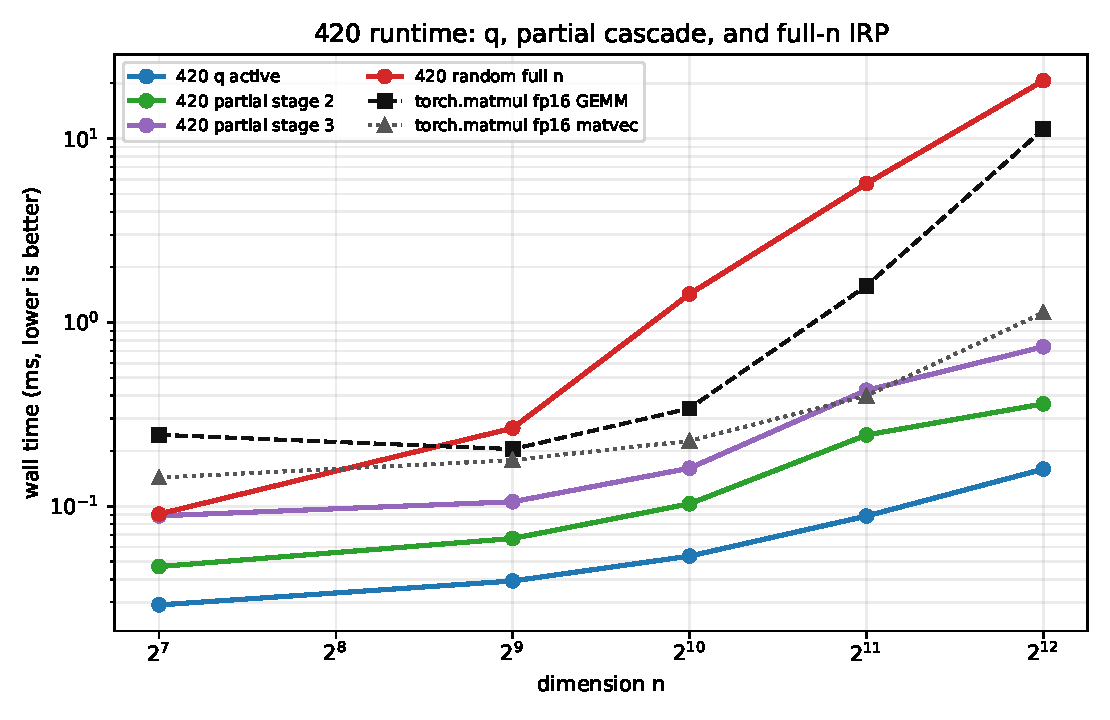
\includegraphics[width=0.96\linewidth]{420_runtime_cascade_vs_matmul.pdf}
\caption{Runtime of 420 across four regimes.  The q-active and partial-cascade
families stop in small subspaces and stay far below the dense fp16 GEMM curve at
large \(n\).  The random control reaches full \(n\) and loses to optimized dense
matmul at large sizes.}
\label{fig:runtime}
\end{figure}

\begin{figure}[htbp]
\centering
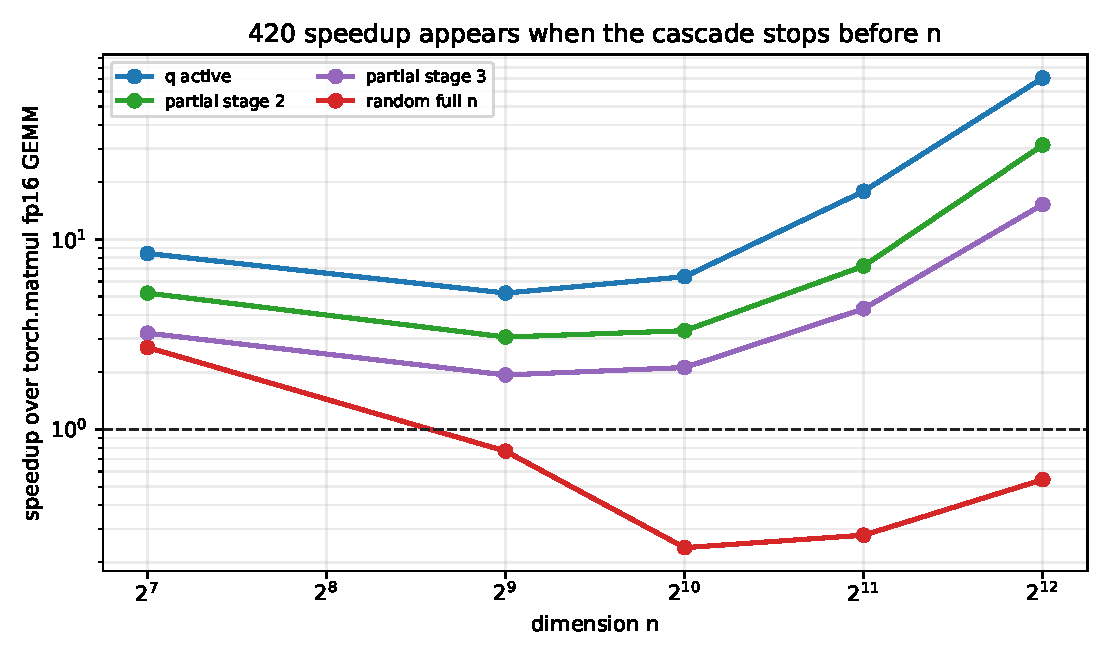
\includegraphics[width=0.90\linewidth]{420_speedup_cascade_vs_fp16_gemm.pdf}
\caption{Speedup over dense fp16 \matmul{} GEMM.  The parity line is at \(1\).
The partial stage 2 and partial stage 3 curves show the main result: the first
\(q\) stage can fail while 420 still wins because the cascade stops well before
\(n\).}
\label{fig:speedup}
\end{figure}

\begin{figure}[htbp]
\centering
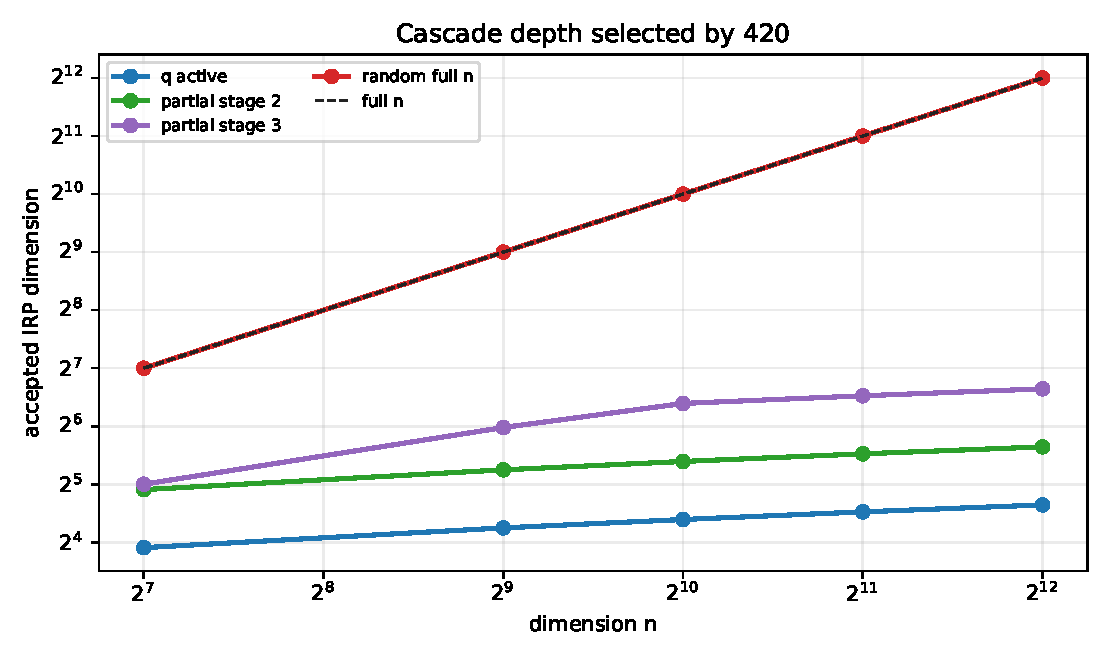
\includegraphics[width=0.90\linewidth]{420_accepted_dimension.pdf}
\caption{Accepted cascade dimension.  The random control follows the full
\(n\) diagonal.  The useful cases stay at dimensions \(q\), \(2q\), or roughly
\(4q/k\), explaining the runtime separation.}
\label{fig:accepted-dim}
\end{figure}

\begin{figure}[htbp]
\centering
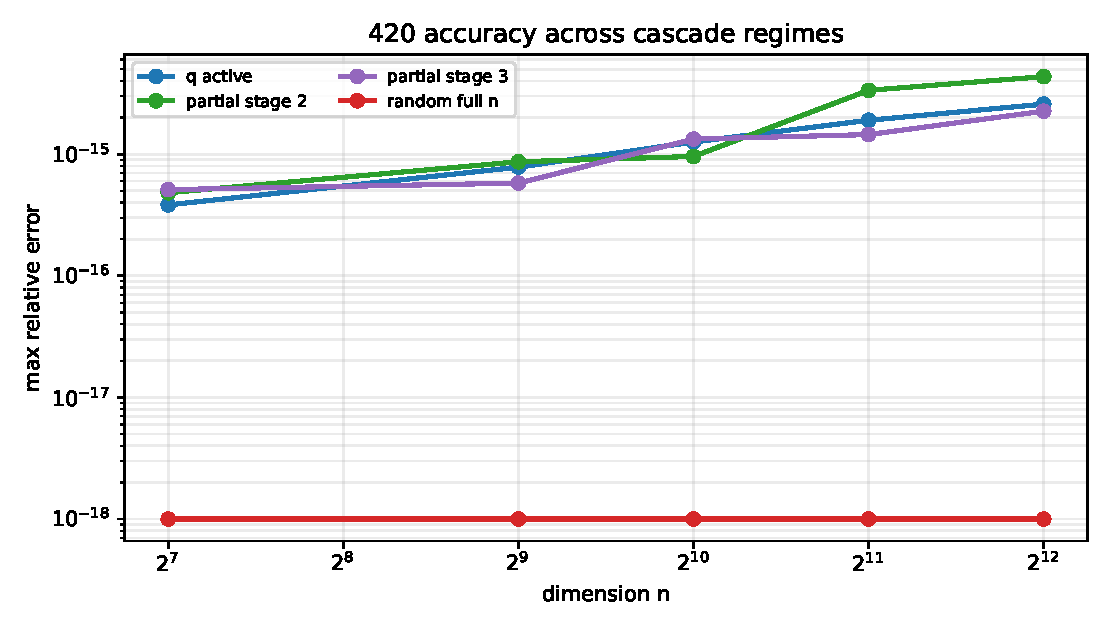
\includegraphics[width=0.90\linewidth]{420_relative_error.pdf}
\caption{Maximum relative error across the three seeds.  The q-active and
partial-cascade rows remain near floating-point precision; the random identity
rows are exact in the reported metric because the full-\(n\) identity projection
is reached.}
\label{fig:error}
\end{figure}

\begin{table}[htbp]
\centering
\scriptsize
\resizebox{\linewidth}{!}{%
\begin{tabular}{llrrrrrrrr}
\toprule
family & \(n\) & \(q/k\) & accepted dim & 420 ms & GEMM fp16 ms & GEMM speed &
matvec fp16 ms & matvec speed & max rel. err.\\
\midrule
\CascadeTableRows
\bottomrule
\end{tabular}}
\caption{Main 420 benchmark rows.  Speed values are baseline time divided by
420 time; values above \(1\) mean 420 is faster.}
\label{tab:main}
\end{table}

\section{Middle-cascade regime}

The middle-cascade rows are the decisive experiment for 420.  They are not
first-stage \qpath{} wins, and they are not full-\(n\) rescues.  They test the
case where \(q\) is too small but a slightly larger IRP subspace is enough.

\begin{table}[htbp]
\centering
\scriptsize
\resizebox{\linewidth}{!}{%
\begin{tabular}{llrrrrrrr}
\toprule
family & \(n\) & \(q/k\) & expected dim & accepted dim & 420 ms &
GEMM speed & matvec speed & max rel. err.\\
\midrule
\MiddleCascadeRows
\bottomrule
\end{tabular}}
\caption{Partial cascade rows.  Stage 2 uses about \(2q\); stage 3 uses about
\(4q\) or the full sketch \(k\), still far below \(n\) for large systems.}
\label{tab:middle}
\end{table}

At \(n=\PtwoBestN\), partial stage 2 accepts dimension \(\PtwoBestDim\) and
reaches \(\PtwoBestSpeedup\times\) over fp16 GEMM, with maximum relative error
\(\PtwoMaxRelError\).  At \(n=\PthreeBestN\), partial stage 3 accepts dimension
\(\PthreeBestDim\) and still reaches \(\PthreeBestSpeedup\times\), with maximum
relative error \(\PthreeMaxRelError\).

\section{Negative control}

The random family is included to prevent overclaiming.  In this case the target
does not have a low-dimensional cascade representation, so 420 must go to the
final full-\(n\) IRP stage.

\begin{table}[htbp]
\centering
\scriptsize
\begin{tabular}{llrrrrrr}
\toprule
family & \(n\) & \(q/k\) & accepted dim & 420 ms & GEMM speed & matvec speed &
max rel. err.\\
\midrule
\RandomControlRows
\bottomrule
\end{tabular}
\caption{Random dense control.  420 remains no-fallback and accurate, but it no
longer keeps the algorithmic advantage.}
\label{tab:random}
\end{table}

This table is the honest boundary of the claim.  420 is reliable without
fallback, but reliability in the dense unstructured case is obtained by paying
the full-dimensional IRP cost.

\section{Interpretation}

The benchmark supports three claims.

\begin{enumerate}[leftmargin=1.4em]
\item \textbf{No-fallback correctness is feasible.}  420 does not need to exit
to a dense external fallback when the first \(q\)-stage fails.  It can keep
growing the IRP space until the residual is solved.
\item \textbf{The useful speed regime is broader than the first \qpath.}
Partial stage 2 and partial stage 3 remain fast because their accepted
dimensions are still much smaller than \(n\).
\item \textbf{There is no free lunch for dense random targets.}  When the
intrinsic dimension is \(n\), 420 reaches \(n\), and dense \matmul{} becomes the
right baseline.
\end{enumerate}

Thus the best formulation is not ``420 beats matmul universally''.  The
defensible formulation is:
\[
\boxed{
\begin{minipage}{0.82\linewidth}
\centering
420 solves by full Pandrosion IRP without fallback, and wins when the accepted
cascade dimension is small.
\end{minipage}}
\]

\section{Limitations and next steps}

The present benchmark is a controlled identity-target study.  It isolates the
cascade mechanism cleanly, but it is not yet a full AI workload benchmark.  The
main missing items are:
\begin{itemize}[leftmargin=1.2em]
\item CUDA/Tensor Core measurements on NVIDIA GPUs;
\item real transformer/adapter workloads using 420's cascade criterion;
\item statistical sweeps with more seeds and noisy near-cascade targets;
\item comparison against classical low-rank, randomized sketching, and block
low-rank methods;
\item a PyTorch-native 420 implementation to reduce Python/NumPy overhead while
keeping the no-fallback IRP design.
\end{itemize}

\section{Conclusion}

Pandrosion 420 turns the \qpath{} from an all-or-nothing event into a cascade.
If the first coded subspace is too small, 420 grows the correction space and
continues inside IRP.  The measured results show that this middle regime is
valuable: stage 2 and stage 3 can still beat dense \matmul{} by large factors
while preserving near-machine-precision accuracy.  The method remains honest in
the random dense case: it solves without fallback, but it no longer claims a
speed advantage.

\end{document}
